\documentclass[svgnames,tikz]{standalone}

\def\unit{5}

\begin{document}
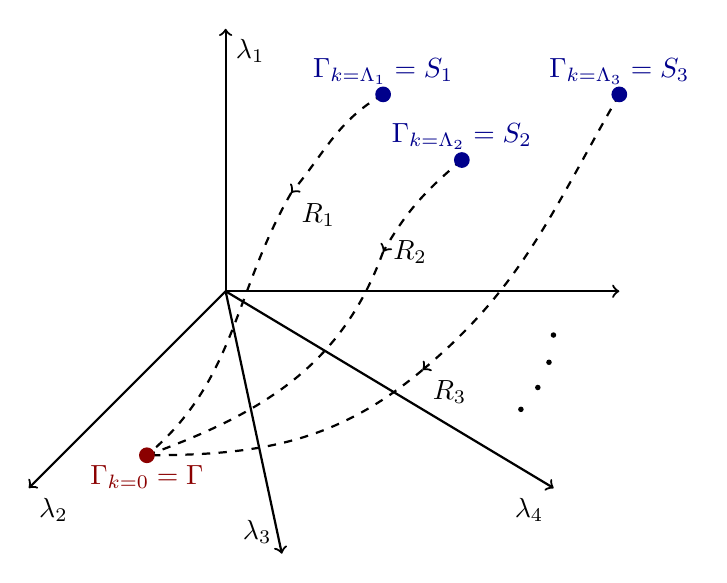
\begin{tikzpicture}[thick]

  % Coordinates of initial, end and midpoints of transition to complexity
  \coordinate (qea) at (-1/5*\unit,-5/12*\unit); %quantum effective action
  \coordinate (ma1) at (2/5*\unit,1/2*\unit); %microscopic action 1
  \coordinate (ma2) at (3/5*\unit,1/3*\unit); %microscopic action 2
  \coordinate (ma3) at (\unit,1/2*\unit); %microscopic action 3
  \coordinate (r1) at (1/6*\unit,1/4*\unit); %regulator 1
  \coordinate (r2) at (2/5*\unit,1/10*\unit); %regulator 2
  \coordinate (r3) at (1/2*\unit,-1/5*\unit); %regulator 3

  % Coordinate system
  \draw[->] (0,0) -- (0,2/3*\unit) node[below right] (l1) {$\lambda_1$};
  \draw[->] (0,0) -- (-1/2*\unit,-1/2*\unit) node[below right] (l2) {$\lambda_2$};
  \draw[->] (0,0) -- (1/7*\unit,-2/3*\unit) node[above left] (l3) {$\lambda_3$};
  \draw[->] (0,0) -- (5/6*\unit,-1/2*\unit) node[below left] (l4) {$\lambda_4$};
  \draw[->] (0,0) -- (\unit,0);
  \draw[line width=2,line cap=round,dash pattern=on 0pt off 5\pgflinewidth] (3/4*\unit,-3/10*\unit) edge[bend right=20] (5/6*\unit,-1/10*\unit);

  % Flow trajectories
  \draw[dashed] (ma1) edge[->,in=50,out=210] (r1) (r1) node[below right] {$R_1$} to[out=240,in=40] (qea);
  \draw[dashed] (ma2) edge[->,in=60,out=220] (r2) (r2) node[right] {$R_2$} to[out=250,in=20] (qea);
  \draw[dashed] (ma3) edge[->,in=40,out=240] (r3) (r3) node[below right] {$R_3$} to[out=220,in=0] (qea);

  % Initial and end points
  \fill[DarkRed] (qea) circle (0.1) node[below] {$\Gamma_{k=0} = \Gamma$};
  \fill[DarkBlue] (ma1) circle (0.1) node[above] {$\Gamma_{k=\Lambda_1} = S_1$};
  \fill[DarkBlue] (ma2) circle (0.1) node[above] {$\Gamma_{k=\Lambda_2} = S_2$};
  \fill[DarkBlue] (ma3) circle (0.1) node[above] {$\Gamma_{k=\Lambda_3} = S_3$};

\end{tikzpicture}
\end{document}
